\documentclass{article}\usepackage{graphicx, color}
%% maxwidth is the original width if it is less than linewidth
%% otherwise use linewidth (to make sure the graphics do not exceed the margin)
\makeatletter
\def\maxwidth{ %
  \ifdim\Gin@nat@width>\linewidth
    \linewidth
  \else
    \Gin@nat@width
  \fi
}
\makeatother

\definecolor{fgcolor}{rgb}{0.2, 0.2, 0.2}
\newcommand{\hlnumber}[1]{\textcolor[rgb]{0,0,0}{#1}}%
\newcommand{\hlfunctioncall}[1]{\textcolor[rgb]{0.501960784313725,0,0.329411764705882}{\textbf{#1}}}%
\newcommand{\hlstring}[1]{\textcolor[rgb]{0.6,0.6,1}{#1}}%
\newcommand{\hlkeyword}[1]{\textcolor[rgb]{0,0,0}{\textbf{#1}}}%
\newcommand{\hlargument}[1]{\textcolor[rgb]{0.690196078431373,0.250980392156863,0.0196078431372549}{#1}}%
\newcommand{\hlcomment}[1]{\textcolor[rgb]{0.180392156862745,0.6,0.341176470588235}{#1}}%
\newcommand{\hlroxygencomment}[1]{\textcolor[rgb]{0.43921568627451,0.47843137254902,0.701960784313725}{#1}}%
\newcommand{\hlformalargs}[1]{\textcolor[rgb]{0.690196078431373,0.250980392156863,0.0196078431372549}{#1}}%
\newcommand{\hleqformalargs}[1]{\textcolor[rgb]{0.690196078431373,0.250980392156863,0.0196078431372549}{#1}}%
\newcommand{\hlassignement}[1]{\textcolor[rgb]{0,0,0}{\textbf{#1}}}%
\newcommand{\hlpackage}[1]{\textcolor[rgb]{0.588235294117647,0.709803921568627,0.145098039215686}{#1}}%
\newcommand{\hlslot}[1]{\textit{#1}}%
\newcommand{\hlsymbol}[1]{\textcolor[rgb]{0,0,0}{#1}}%
\newcommand{\hlprompt}[1]{\textcolor[rgb]{0.2,0.2,0.2}{#1}}%

\usepackage{framed}
\makeatletter
\newenvironment{kframe}{%
 \def\at@end@of@kframe{}%
 \ifinner\ifhmode%
  \def\at@end@of@kframe{\end{minipage}}%
  \begin{minipage}{\columnwidth}%
 \fi\fi%
 \def\FrameCommand##1{\hskip\@totalleftmargin \hskip-\fboxsep
 \colorbox{shadecolor}{##1}\hskip-\fboxsep
     % There is no \\@totalrightmargin, so:
     \hskip-\linewidth \hskip-\@totalleftmargin \hskip\columnwidth}%
 \MakeFramed {\advance\hsize-\width
   \@totalleftmargin\z@ \linewidth\hsize
   \@setminipage}}%
 {\par\unskip\endMakeFramed%
 \at@end@of@kframe}
\makeatother

\definecolor{shadecolor}{rgb}{.97, .97, .97}
\definecolor{messagecolor}{rgb}{0, 0, 0}
\definecolor{warningcolor}{rgb}{1, 0, 1}
\definecolor{errorcolor}{rgb}{1, 0, 0}
\newenvironment{knitrout}{}{} % an empty environment to be redefined in TeX

\usepackage{alltt}
\usepackage{mathtools}
\usepackage{amsfonts}
\usepackage{subfig}
%\VignetteEngine{knitr}
%\VignetteIndexEntry{}
\IfFileExists{upquote.sty}{\usepackage{upquote}}{}

\begin{document}
\title{randPort vignette}
\author{Mike Flynn, Angel Zhou, Dave Kane}
\maketitle

\section*{Sampling from Linear Inverse problems}




A simple case to consider is one with only 3 stocks in the universe, say GE, IBM and Coca-Cola (KO). Assume that there is some data available about these stocks:

\begin{knitrout}
\definecolor{shadecolor}{rgb}{0.969, 0.969, 0.969}\color{fgcolor}\begin{kframe}
\begin{alltt}
\hlfunctioncall{set.seed}(40)
stocks <- \hlfunctioncall{data.frame}(ticker = \hlfunctioncall{c}(\hlstring{"GE"}, \hlstring{"IBM"}, \hlstring{"KO"}), sizerank = \hlfunctioncall{c}(1, 0, -1))
stocks
\end{alltt}
\begin{verbatim}
##   ticker sizerank
## 1     GE        1
## 2    IBM        0
## 3     KO       -1
\end{verbatim}
\end{kframe}
\end{knitrout}


The most basic constraint is the long-only constraint i.e. the weights of the stock must add up to one and be positive. This can be represented by a linear equation: let the weights of ``GE",``IBM", and ``KO", be $x$, $y$, and $z$, respectively. Then $x+y+z =1$, $x,y,z \ge 0$ are the only constraints. The \verb+randPort+ package is designed to sample underdetermined equations of the form $Ax=b$, with $x \ge 0$ and so it is ideal for this set of constraints. In this case $A = [1,1,1]$ and $b = 1$. With \verb+hitandrun+, we can easily obtain a set of weights that are randomly distributed and fulfill the constraints. 

\begin{knitrout}
\definecolor{shadecolor}{rgb}{0.969, 0.969, 0.969}\color{fgcolor}\begin{kframe}
\begin{alltt}
A <- \hlfunctioncall{matrix}(\hlfunctioncall{c}(1, 1, 1), nrow = 1, ncol = 3)
A
\end{alltt}
\begin{verbatim}
##      [,1] [,2] [,3]
## [1,]    1    1    1
\end{verbatim}
\begin{alltt}
b <- 1

w <- \hlfunctioncall{hitandrun}(A, b, n = 1000)
points <- \hlfunctioncall{as.data.frame}(\hlfunctioncall{t}(w))
\hlfunctioncall{colnames}(points) <- stocks$ticker
\hlfunctioncall{head}(points)
\end{alltt}
\begin{verbatim}
##        GE     IBM     KO
## 1 0.10506 0.03877 0.8562
## 2 0.07990 0.83320 0.0869
## 3 0.09234 0.80191 0.1057
## 4 0.14397 0.44635 0.4097
## 5 0.43460 0.26308 0.3023
## 6 0.13072 0.19263 0.6766
\end{verbatim}
\end{kframe}
\end{knitrout}





The pairwise scatters display the fact that any pair of variables has a sum bounded by 1, but can be anywhere between that line and the axes. 

\begin{figure}[t]
\begin{knitrout}
\definecolor{shadecolor}{rgb}{0.969, 0.969, 0.969}\color{fgcolor}
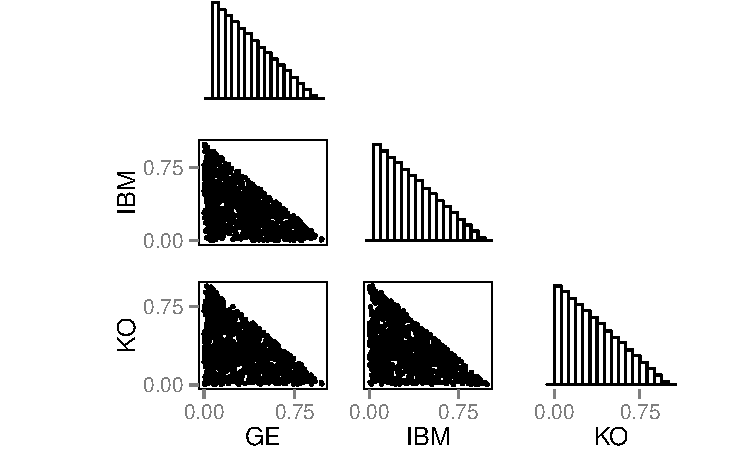
\includegraphics[width=\maxwidth]{figure/figChunk1} 

\end{knitrout}

\caption{Consider the case with 3 stocks. The only constraint is that we are fully invested and long-only. For the scatterplots, 1000 random portfolios were sampled. For the histograms, 100,000 samples were taken to increase resolution. Because each stock is exchangeable in the current scheme, we should have that all their weight distributions are identical. For each stock the probability density of its weight decreases linearly as the weight increases. The reason is as follows: each variable is a function of the other 2. For example: let $x$ be GE, $y$-IBM, and $z$-KO. We know $z = 1 - (x+y)$. The most probable value of $(x+y)$ corresponds to the line $y= c-x$ with the most points on it, the longest line. As can be seen in the distributions, the longest such line is $y=1-x$, therefore the most probable value for $x+y$ is 1 and the most probable value for $z$ is 0, and likewise for $x$ and $y$.}
\end{figure}

Perhaps now we want to match a portfolio that has an exposure to size rank of 0.5. This is the same thing as adding a new row to A and b, corresponding to the column ``sizerank" of our stock data and 0.5 respectively.

\begin{knitrout}
\definecolor{shadecolor}{rgb}{0.969, 0.969, 0.969}\color{fgcolor}\begin{kframe}
\begin{alltt}
A <- \hlfunctioncall{rbind}(A, stocks$sizerank)
b <- \hlfunctioncall{c}(b, 0)

w3 <- \hlfunctioncall{hitandrun}(A, b, n = 1000)
points3 <- \hlfunctioncall{as.data.frame}(\hlfunctioncall{t}(w3))
\hlfunctioncall{colnames}(points3) <- \hlfunctioncall{colnames}(points)
\hlfunctioncall{head}(points3)
\end{alltt}
\begin{verbatim}
##        GE    IBM      KO
## 1 0.25915 0.4817 0.25915
## 2 0.12576 0.7485 0.12576
## 3 0.07995 0.8401 0.07995
## 4 0.02807 0.9439 0.02807
## 5 0.40548 0.1890 0.40548
## 6 0.05422 0.8916 0.05422
\end{verbatim}
\end{kframe}
\end{knitrout}





Running this code is equivalent to sampling from the positive solution space of $x+y+z = 1$ and $x-z = 0$, which corresponds to the line segment paramterized by $r(t) = [t, 1 - 2t, t]$ with $0 \le t \le 0.5$. This is very clear when looking at pairwise plots of the variables.

\begin{figure}[b]
\begin{knitrout}
\definecolor{shadecolor}{rgb}{0.969, 0.969, 0.969}\color{fgcolor}
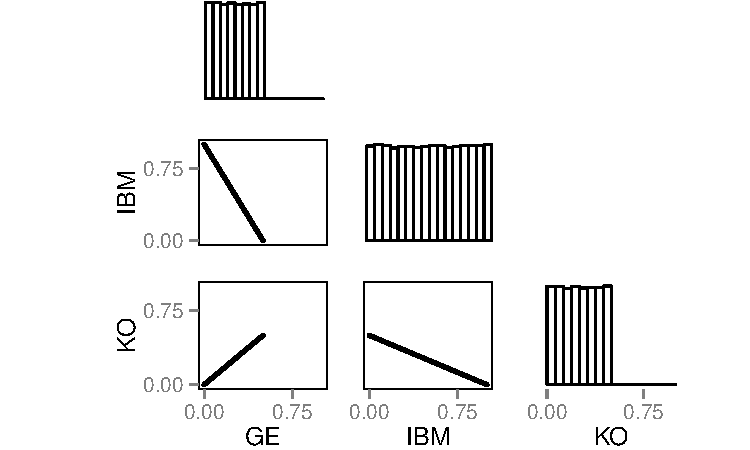
\includegraphics[width=\maxwidth]{figure/plots2} 

\end{knitrout}

\caption{Perhaps we add another constraint that we must be "sizerank" neutral. Again, the scatterplots display 1000 portfolios and the histograms display 100,000. This slices our old plane $x+y+z=1$ by the plane $x - z = 0$. As derived in the text, this curve can be parameterized by $r(t) = [t, 1 - 2t, t]$ with $0 \le t \le 0.5$. This curve can be checked by looking at the pairwise scatter plots (check the end points). Since there is no difference between the number of points at one point of the line vs. another, all the variables are uniformly distributed, however they have different limits, as can be seen by the histograms.}
\end{figure}

\section*{Geometric Nature of the Problem}

It is easier to picture the space of each problem when looking at things geometrically. Each row of Ax=b corresponds to a linear equation $c_1x_1 + c_2x_2 + \dots + c_n x_n = b_m$. Geometrically, this means our solution lies on an (n-1)-plane in $\mathbb{R}^n$. When there are $m$ rows, our solution must lie in the intersection of those $m$ planes which is itself an $(n-m)$ plane. A concrete example is the 3 stock case with no additional constraints. This is the peice of the ($3-1 = 2$)-plane $x+y+z = 1$ that is in the positive quadrant. It forms a triangle. If another constraint is added, it cuts a slice in this triangle, making the valid solution space a line, as you can see via figure \ref{trifig}. When we sample with our function, the random points are distributed uniformly along these shapes. 

Normally we will be dealing with universes much larger than 3 stocks and so the problem becomes harder to picture. The concepts, however, remain the same, we are still just sampling the intersections of planes. In math literature, these shapes are called convex polytopes, and they are very well studied. 

\begin{figure}[h]
\centering

\subfloat[][]{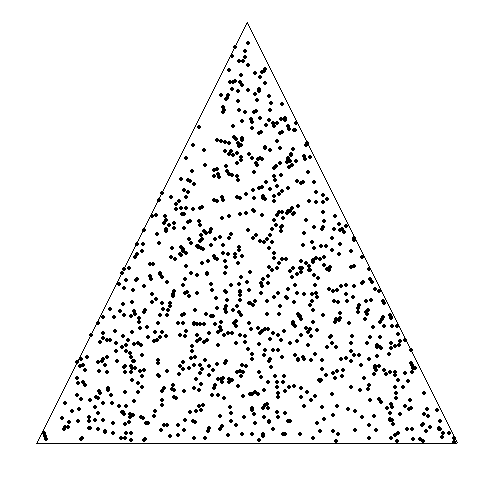
\includegraphics[scale=0.25]{figure/simplex1.png}\label{simplex1}}
\subfloat[][]{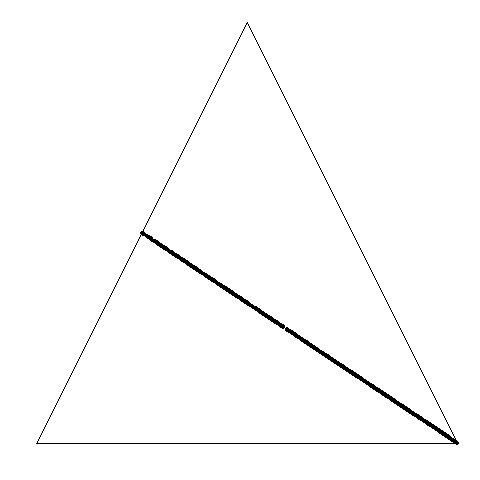
\includegraphics[scale=0.25]{figure/simplex2.png}\label{simplex2}}
\caption{Each vertex of these triangles is a portfolio where we are fully invested in one of the stocks. It is naturally in 3-dimensions, with vertices at $(1,0,0)$, $(0,1,0)$, and $(0,0,1)$, but has been mapped here to 2-dimensions.\\ \protect\subref{simplex1} Here the points only have the constraint that they must add up to 1. As you can see, they are uniformly distributed on this triangle.
 \\ \protect\subref{simplex2} Here we have added the constraint: $x-z=0$. As you can see, only certain points on a line are allowed.Full investment in IBM is allowed because it has a natural exposure to ``sizerank" of 0, and the half and half portfolio with GE and KO is allowed because their average ``sizerank" is 0. The line connecting them is the set of all portfolios fulfilling the constraints and we have sampled them uniformly. It is considerably easier to fully sample a space of smaller dimension.}
 \label{trifig}
\end{figure}

\section*{Algorithm} 




\end{document}
